Quite early in the project it became apparent that a lot of interfacing between the arduino and the individual components would be necessary. 
Thus, we split each functional component up into its own sub-circuit. 
Each sub-circuit is realized on a separate perf-board with pin-headers mounted for external interfacing (see figure \ref{fig:perfboard}). 
The idea is to abstract away power delivery and intermediary connections, such only control pins are routed to the Arduino. 
Power delivery to each board is handled by wires to a common power-distribution board. 
It consists of two XL6009 dc-dc buck-converters, down-stepping the power supply's 24V to 5V and 12V respectively (see figure \ref{fig:powboard}).

\subsection{Schematics}
In table \ref{tab:circuits} the schematics for the primary sub-circuits used in the pinball machine are summarized.

\begin{table*}[h]
	\centering
	\begin{tabular}{@{}lll@{}}
		\toprule
		Circuit & Is shown in & Description \\ \midrule
		\textbf{Flippers}       & Figure  \ref{cir:flipper}  & Reads two buttons and drives two mosFETs.                    \\ 
		\textbf{Popbumpers}     & Figure  \ref{cir:bumper}   & Reads three pieces conductive-tape and drives three mosFETs. \\
		\textbf{Dividers}       & Figure  \ref{cir:top}      & Reads three IR-sensors and controls four LEDs.               \\
		\textbf{Limit-switches} & Figure  \ref{cir:switches} & Reads four switches and controls four LEDs.                  \\
		\textbf{RGB-strip}      & Figure  \ref{cir:rgbled}   & Drives three high-current transistors.                       \\ \bottomrule
	\end{tabular}
	\caption{Circuit index.}
	\label{tab:circuits}
\end{table*}

% ================== POWER =======================
\begin{figure}[h]
	\centering
	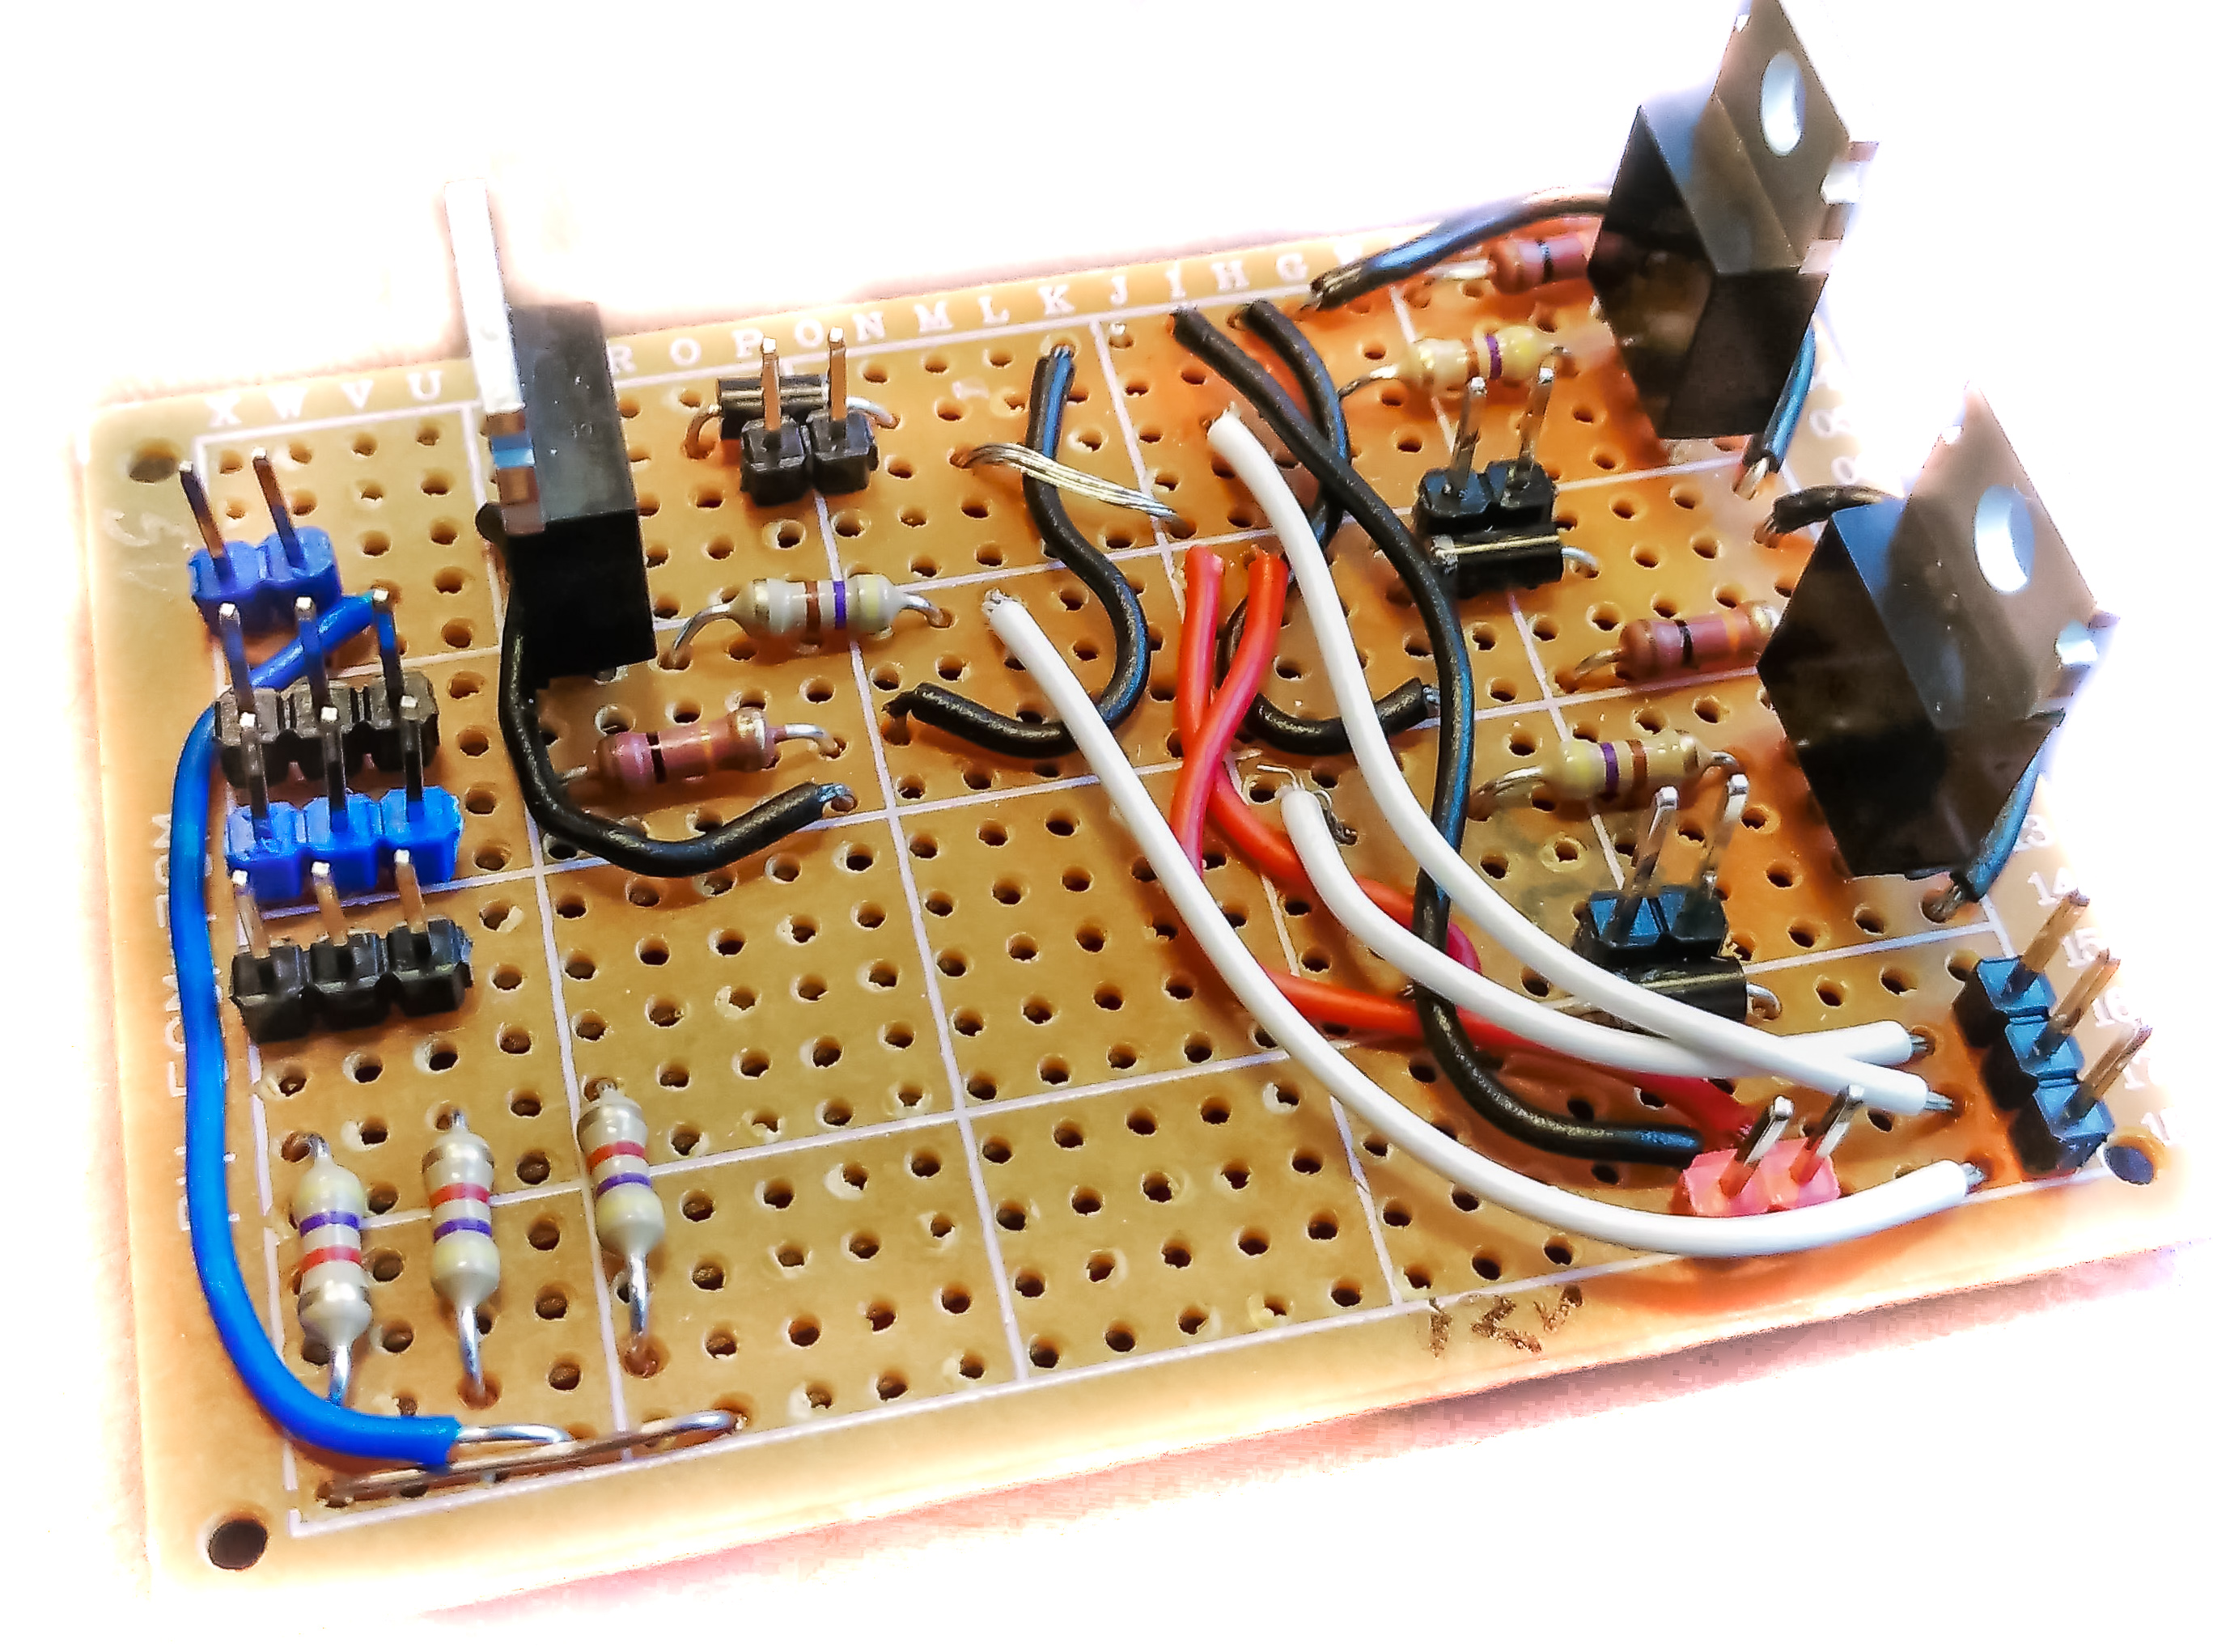
\includegraphics[width=0.42\textwidth]{popbumper_perf}
	\caption{Subcircuit board for controlling the popbumpers.}
	\label{fig:perfboard}
\end{figure}

\begin{figure}[h]
	\centering
	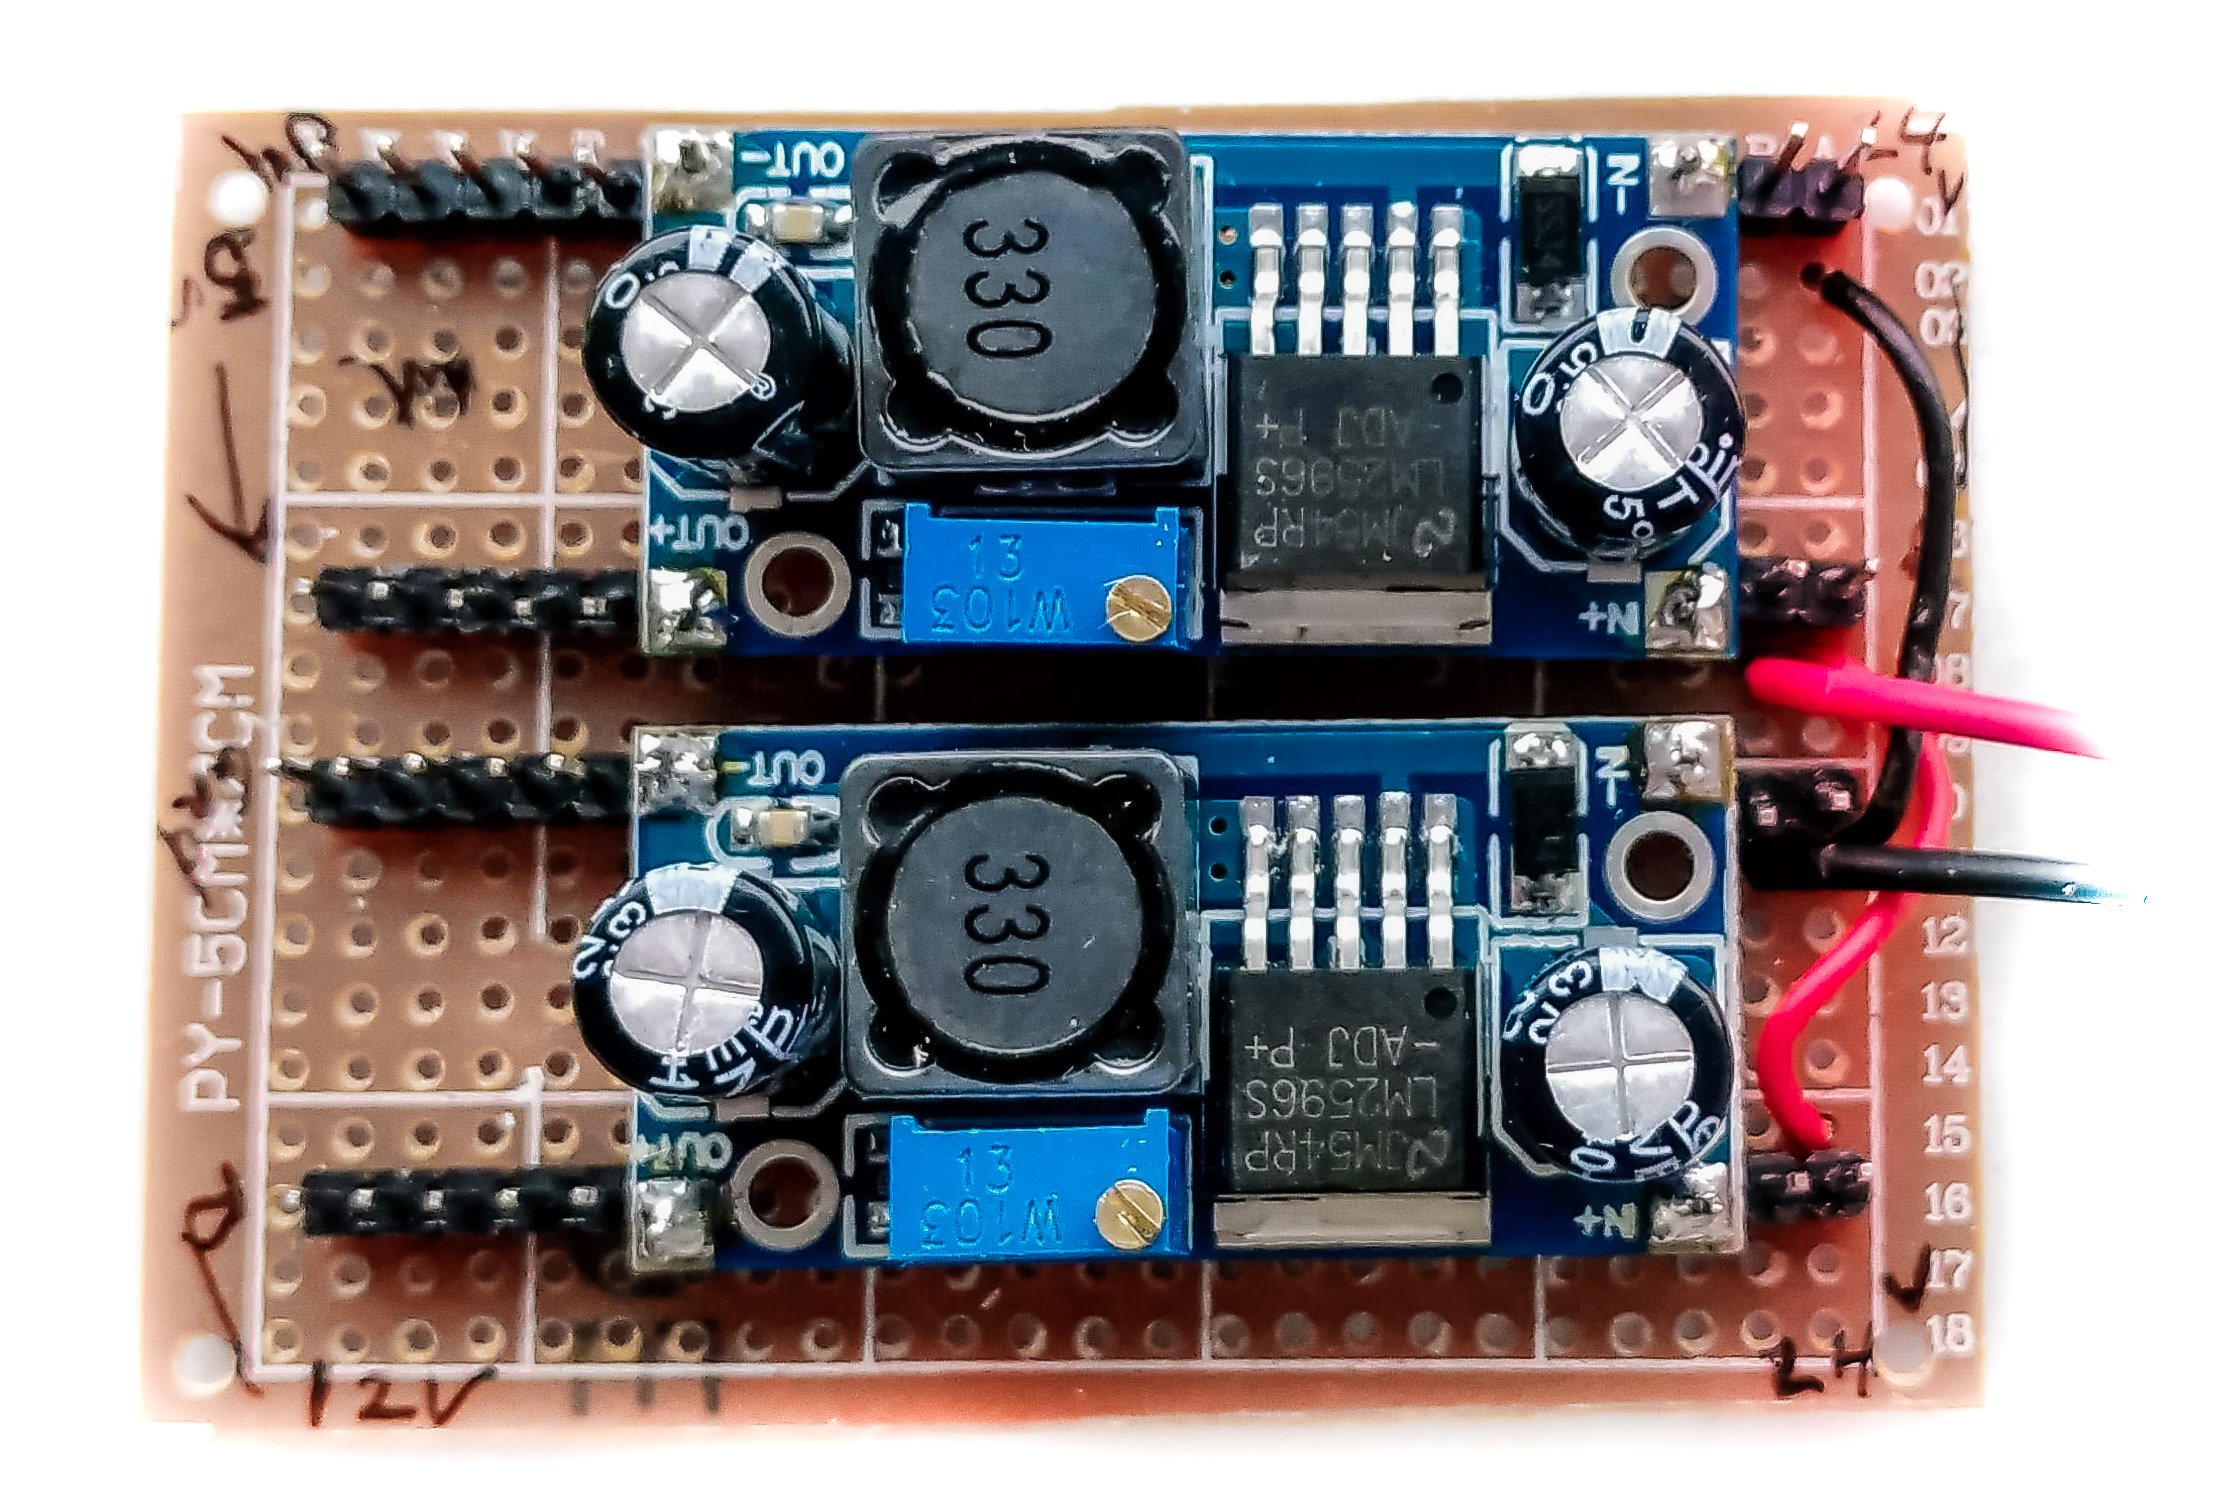
\includegraphics[width=0.42\textwidth]{power_dist}
	\caption{Power distribution board delivering 24V, 12V and 5V to the system.}
	\label{fig:powboard}
\end{figure}

% ================== RGB-LED-COMPONENT =======================
\begin{figure}[h]
	\centering
	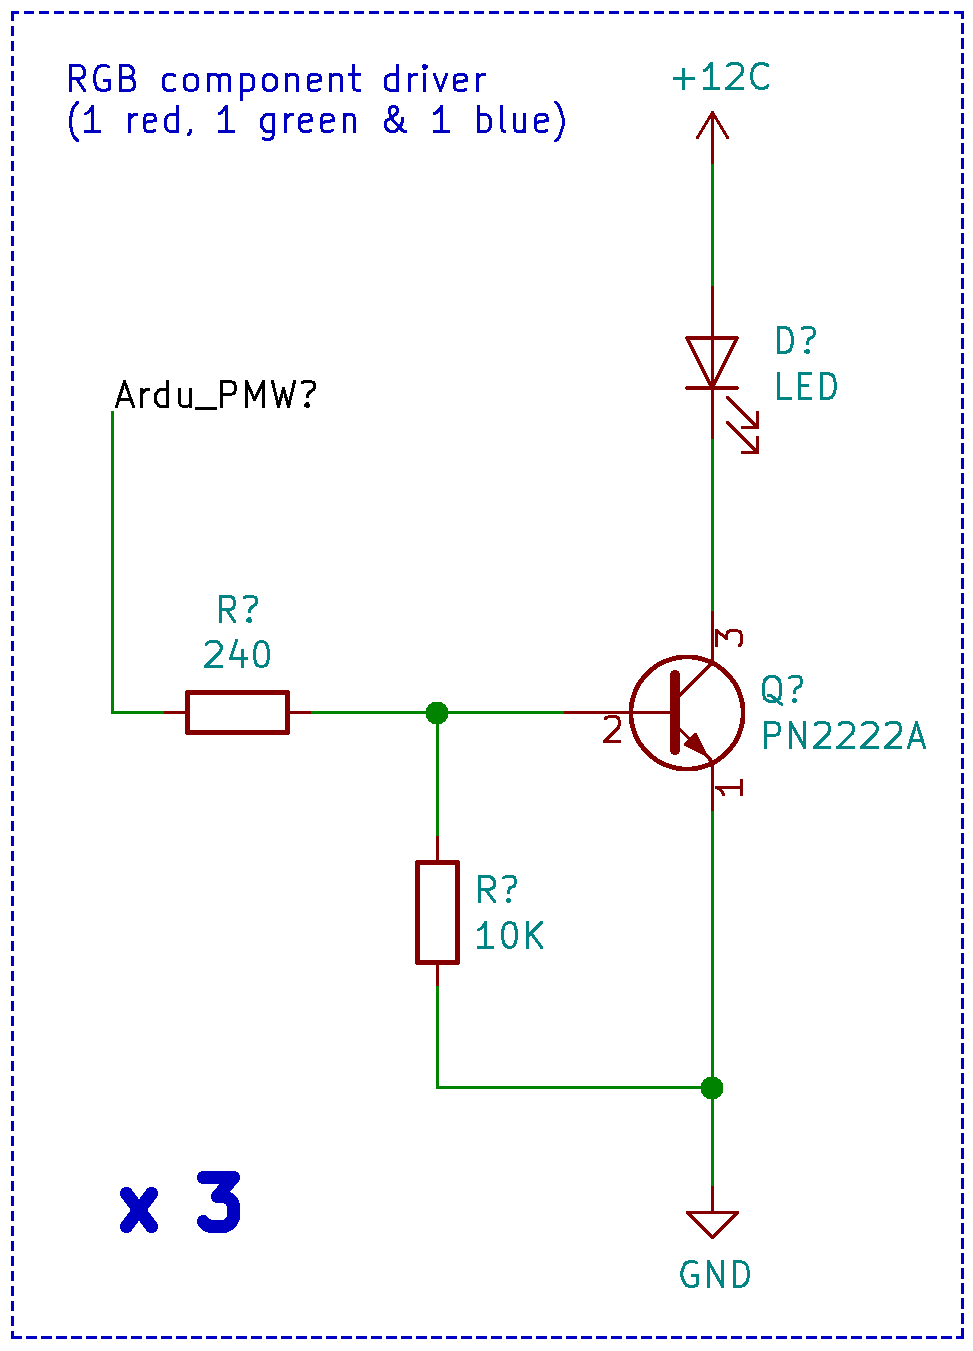
\includegraphics[width=0.38\textwidth]{circuits/rgbled}
	\caption{Schematic of how each color-component of the RGB led strip is driven.}
	\label{cir:rgbled}
\end{figure}

% ================== FLIPPER =======================
\begin{figure*}[h]
	\centering
	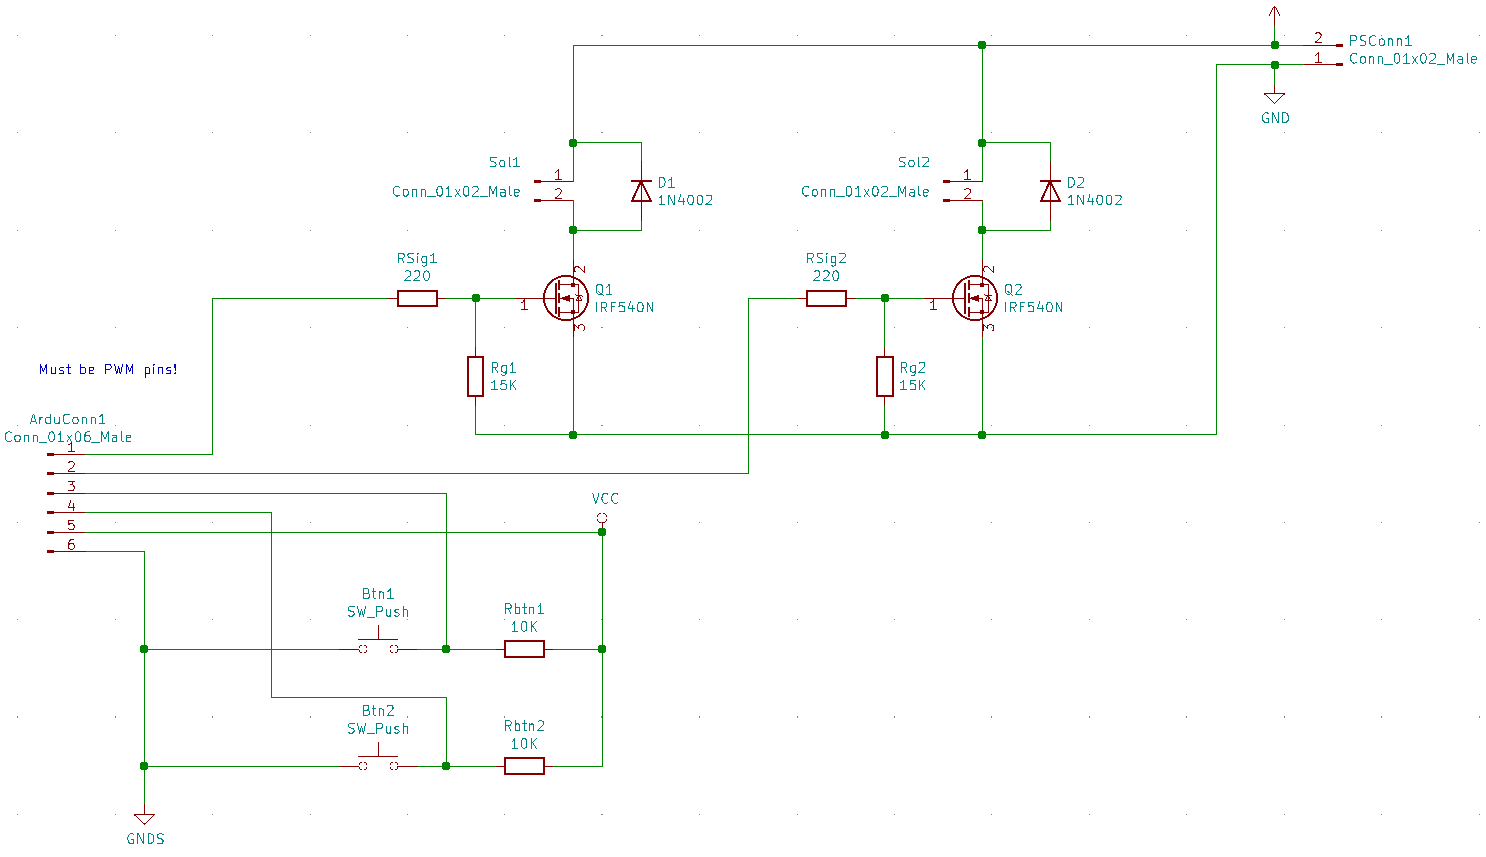
\includegraphics[width=\textwidth]{circuits/flipper}
	\caption{Schematic of the perfboard circuit used to power the flippers.}
	\label{cir:flipper}
\end{figure*}

% ================== BUMPERS =======================
\begin{figure*}[h]
	\centering
	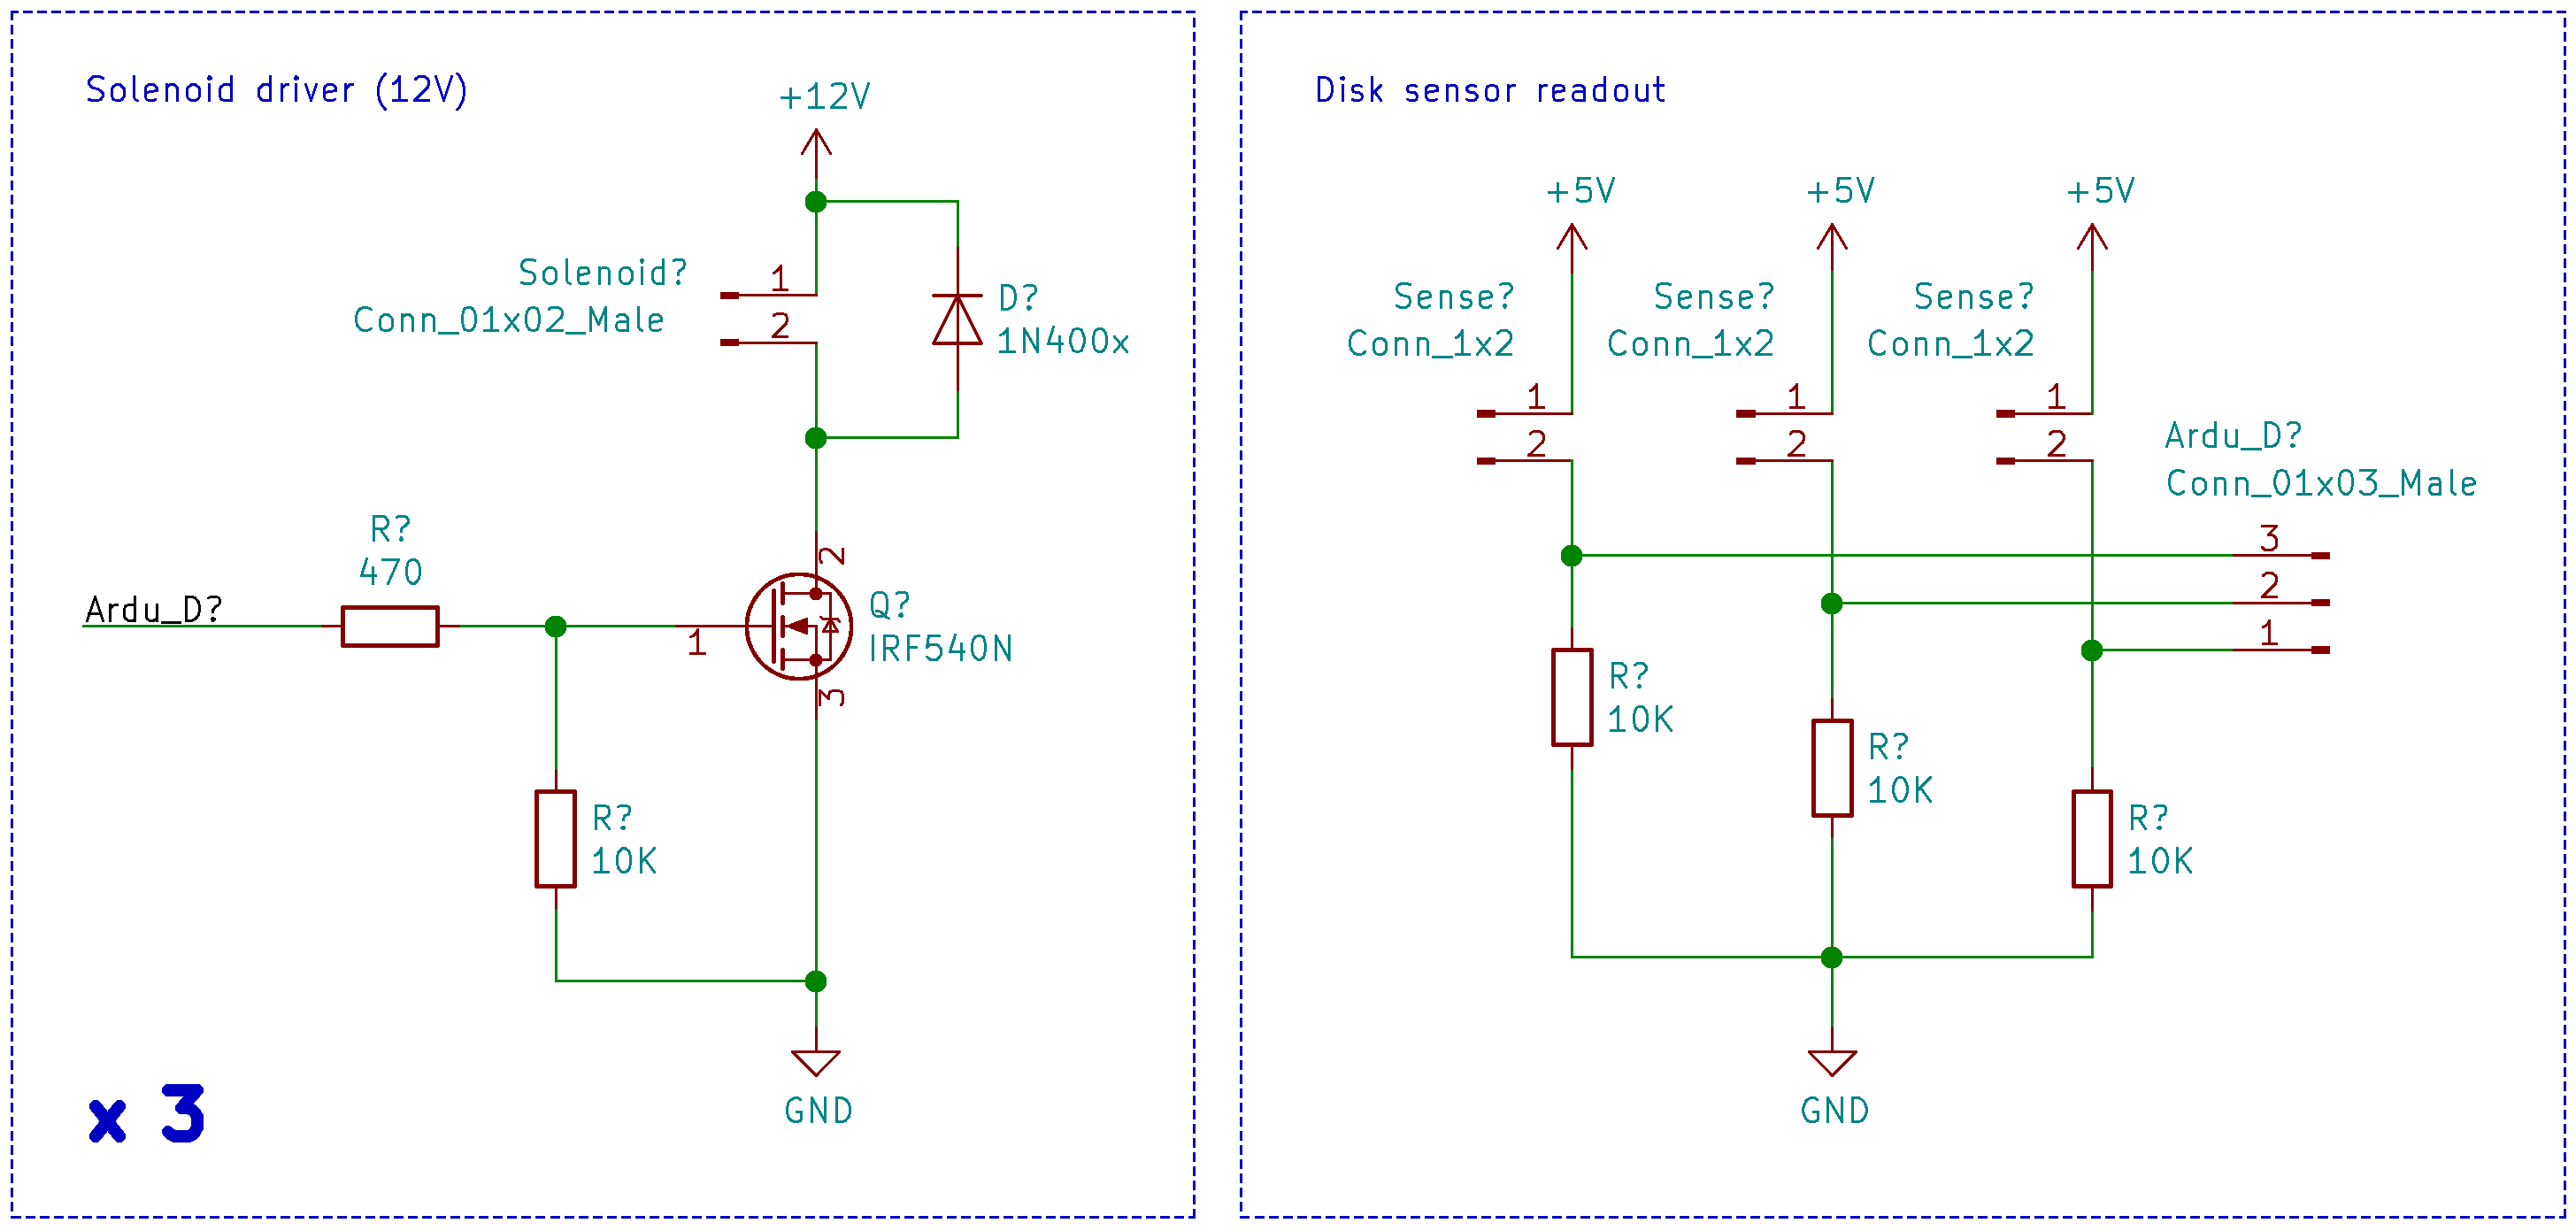
\includegraphics[width=\textwidth]{circuits/popbumper}
	\caption{Schematic of the readout and driver circuit for the pop-bumpers.}
	\label{cir:bumper}
\end{figure*}

% ================== DIVIDERS =======================
\begin{figure*}[h]
	\centering
	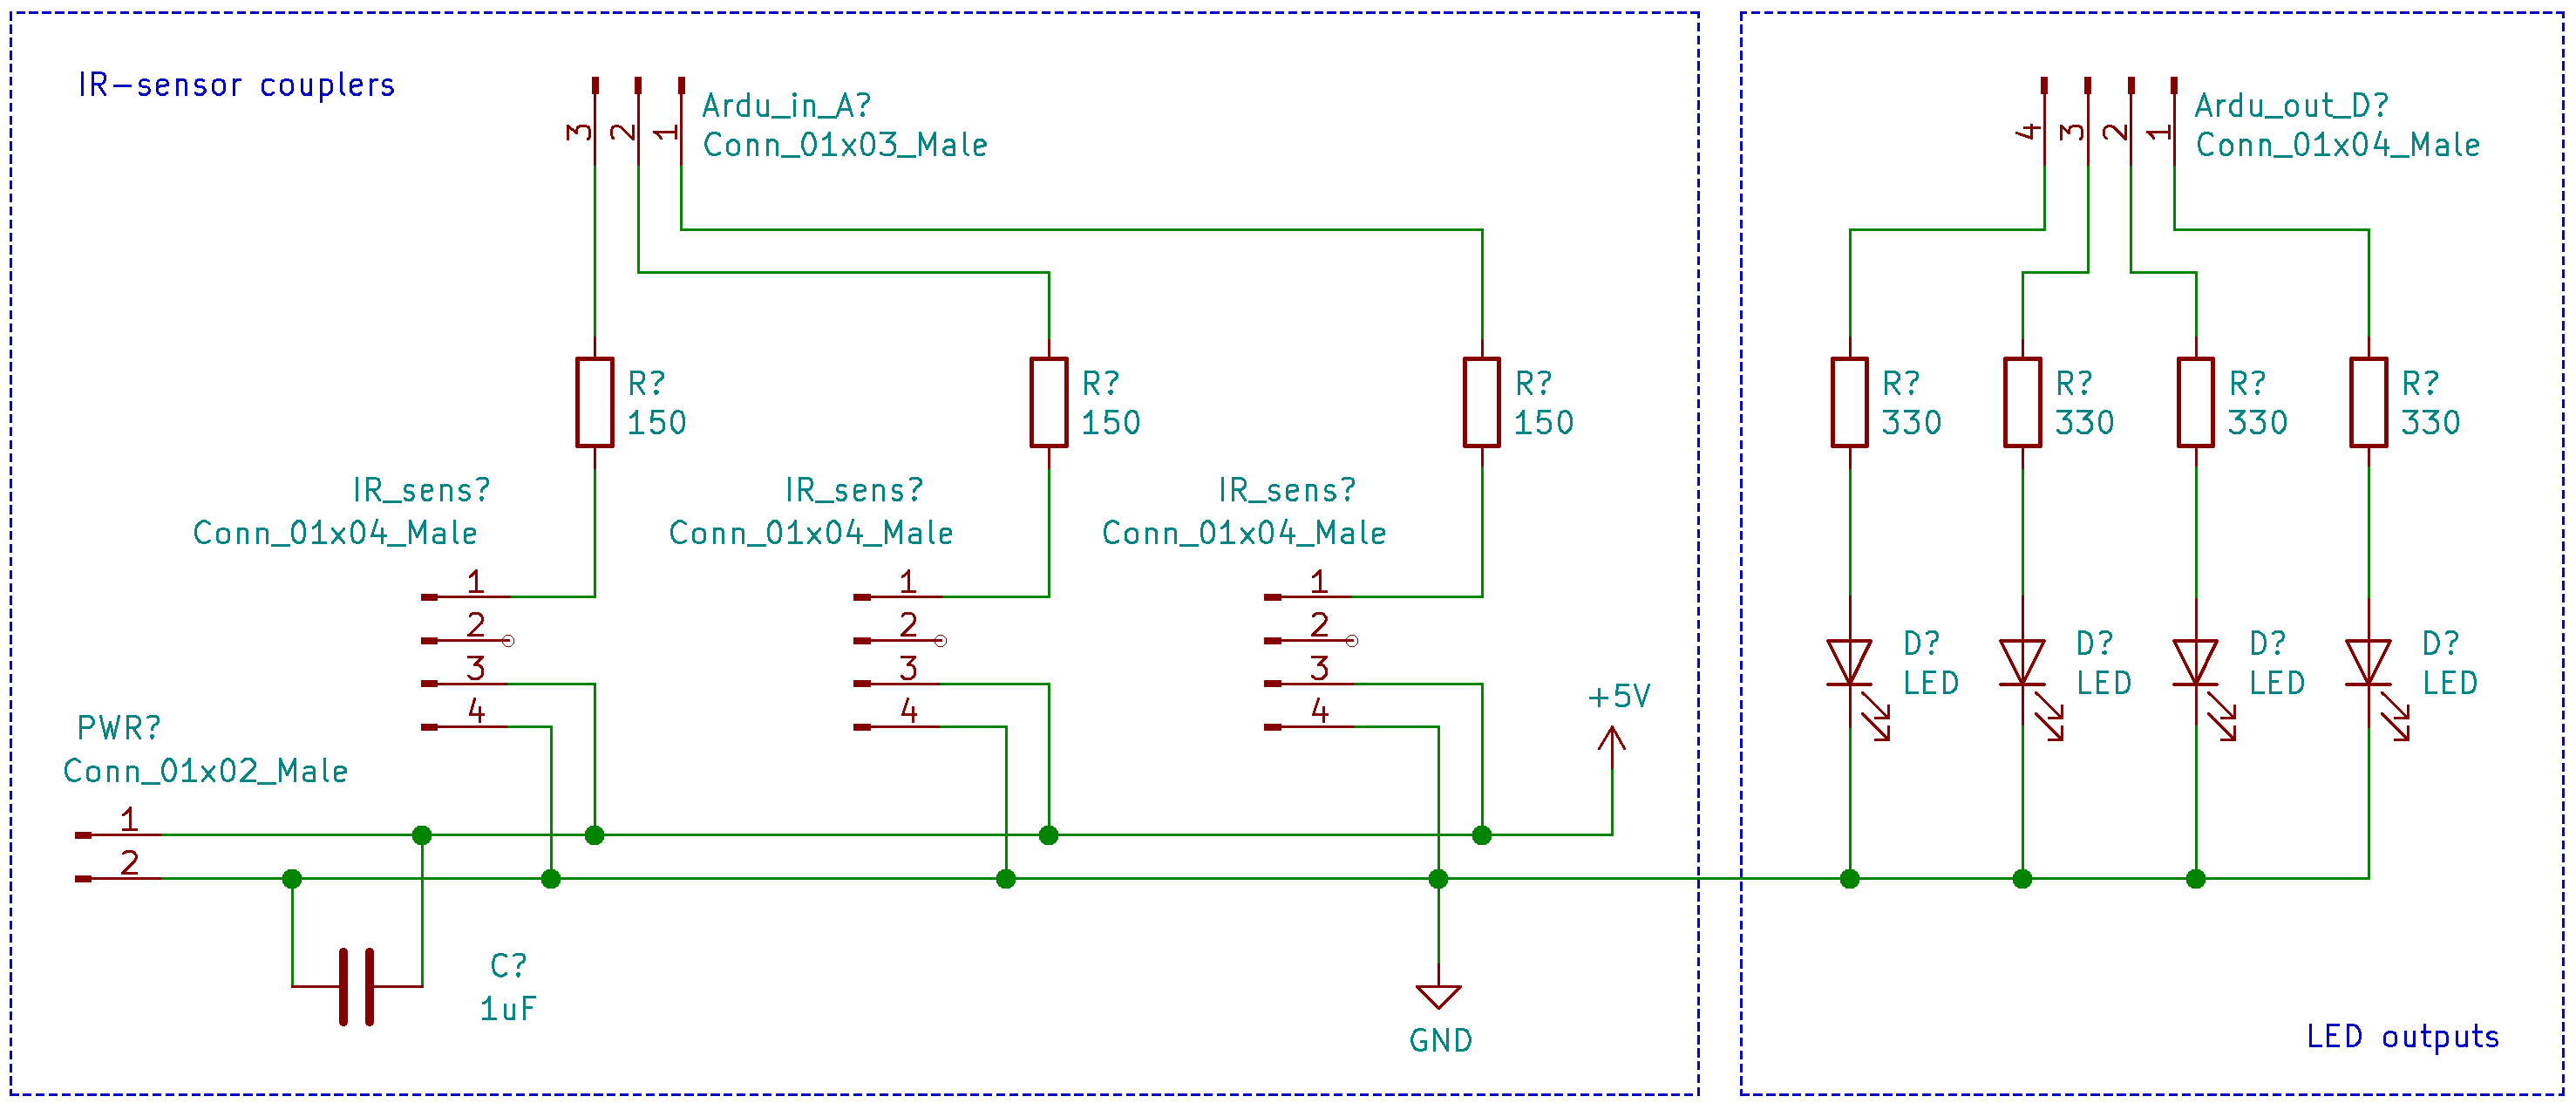
\includegraphics[width=\textwidth]{circuits/toprollers}
	\caption{Schematic of the sensor-coupling and led driver circuit for the top roll-through dividers.}
	\label{cir:top}
\end{figure*}

% ================== LIMIT-SWITCHES =======================
\begin{figure*}[h]
	\centering
	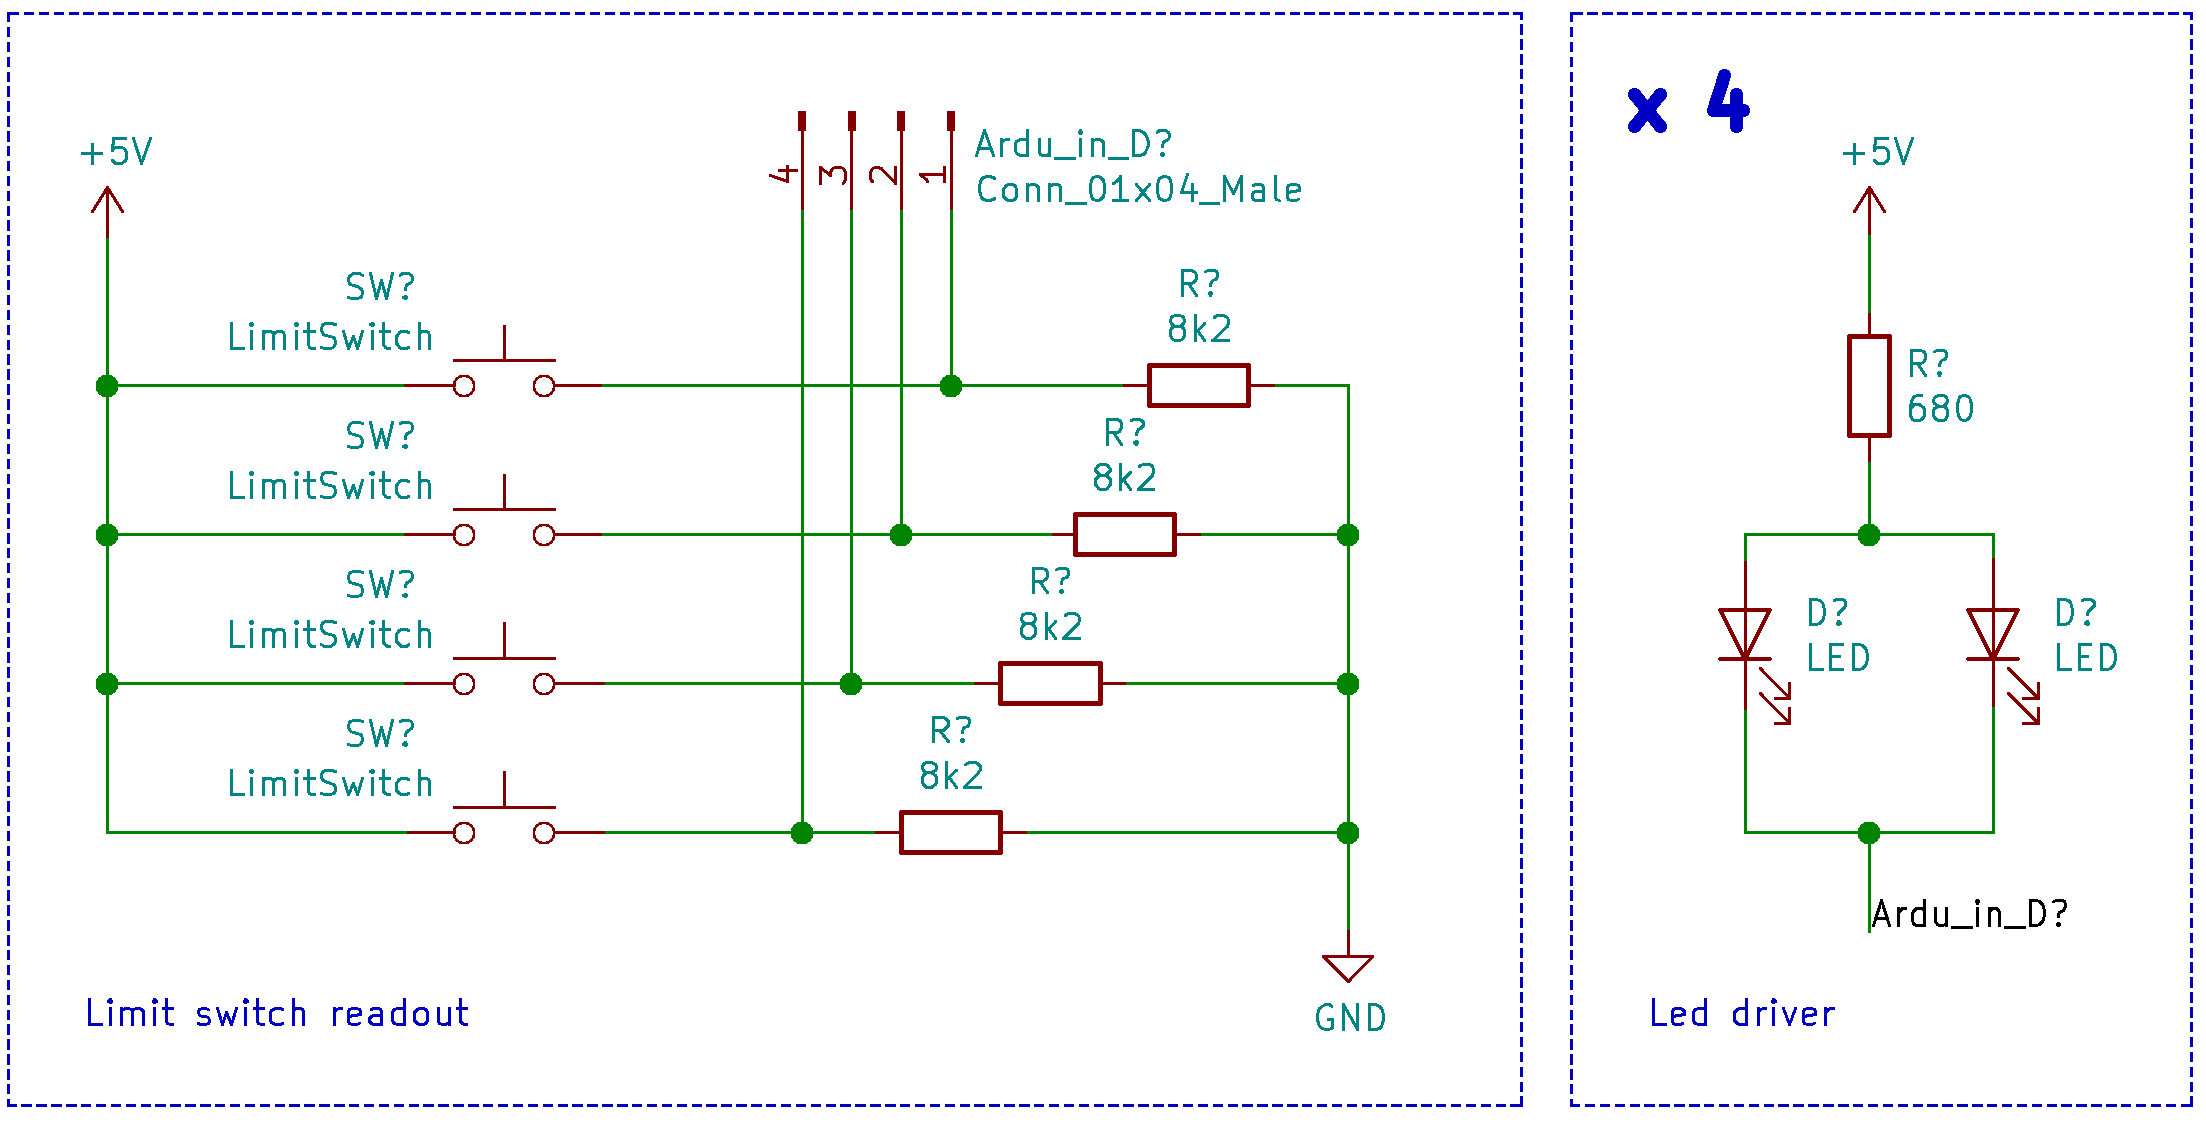
\includegraphics[width=0.8\textwidth]{circuits/limitswitch}
	\caption{Schematic of the limit-switch readout and visual feedback led circuit.}
	\label{cir:switches}
\end{figure*}

